\documentclass[a4paper]{article}

%%%%%%%%%%%%%%%%%%%%%%%%%%%%%%%%%%%%%%%%%%%%%%
\usepackage[T1]{fontenc}
\usepackage{geometry}
\geometry{a4paper,left=1.5cm,right=1cm,top=1cm,bottom=1cm}

\usepackage{graphicx}
\usepackage[absolute,overlay]{textpos}
\usepackage{eso-pic}               % image de fond
\usepackage{fontawesome5}
\usepackage[hidelinks]{hyperref}
\usepackage{tikz}
\usepackage{xcolor}
\usepackage{enumitem}
\setlist{nosep,leftmargin=6mm}
\usepackage{times}                % même police que votre exemple
\usepackage{array} 
\usepackage{tabularx}
\usepackage{ragged2e}
\usepackage{changepage}
\let\origcolorbox\colorbox    % sauvegarde
\renewcommand{\colorbox}[2]{#2}% neutralise le fond
%%%%%%%%%%%%%%%%%%%%%%%%%%%%%%%%%%%%%%%%%%%%%%
%\definecolor{texcolor}{HTML}{e2e8f0}
\providecolor{sidetext}{rgb}{1,1,1}
\definecolor{maincolor}{HTML}{ffffff}

%%%%%%%%%%%%%%%%%%%%%%%%%%%%%%%%%%%%%%%%%
% — Ne changez pas le nom : « background.jpg » doit être présent
\AddToShipoutPictureBG*{%
  
\includegraphics[width=\paperwidth,height=\paperheight]{background.jpg}%
}

%%%%%%%%%%%%%%%%%%%%%%%%%%%%%%%%%%%%%%%%%
\newcommand{\fullrule}{\hspace{-1.5cm}\rule{\paperwidth}{0.4pt}}
\newcommand{\cvsection}[1]{%
  \vspace{6pt}\textbf{\Large #1}\par\vspace{2pt}}
\newcommand{\cicon}[1]{%
  \tikz[baseline]{\draw[fill=white] (0,0.1) circle[radius=0.1cm];}~#1}

\setlength{\parindent}{0pt}
%\color{texcolor}
%%%%%%%%%%%%%%%%%%%%%%%%%%%%%%%%%%%%%%%%%%%%%%%%%%%%%%%%%%%%%%
\begin{document}
\color{white}
% ---------- Photo ------------------------------------------------
\begin{textblock*}{4cm}(0.2cm,0.3cm)
  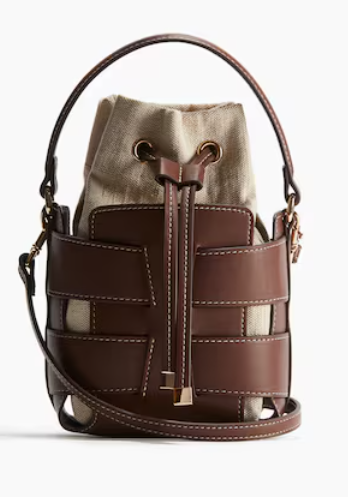
\includegraphics[width=2.5cm,clip,keepaspectratio]{4365698cef6a4b64964dff61591ff191.png}
\end{textblock*}

% ---------- En-tête ---------------------------------------------
\begin{center}
  {\fontsize{44pt}{24pt}\selectfont\bfseries Judikael Mourouvin}

  \bigskip
  {\Large Technicien support \& marketing digital}

  \bigskip\bigskip
  \faMapMarker~Route de Cocoyer\ 97190 Gosier
  \quad\faEnvelope~\href{mailto:jkmou971@gmail.com}{jkmou971@gmail.com}

  \bigskip
  % Badge LinkedIn (retirez-le si inutile)
  \faPhone~ +590 690 91 14 48
  \quad \faLinkedin\ \href{}{}
 

  \vspace{-0.3cm}
  \fullrule
\end{center}

% ---------- Profil ----------------------------------------------
\cvsection{Profil}
\hspace*{2.2cm}%
Passionné par les technologies et la communication en ligne, j’allie des compétences techniques pointues à une vraie sensibilité marketing. J’ai renforcé mon expertise lors d’une année d’alternance à la DSI de la Mairie du Gosier, où j’ai mené des projets numériques et formé les utilisateurs. Curieux et méthodique, je sais diagnostiquer les incidents, maintenir un parc informatique et déployer des solutions digitales adaptées. Je souhaite désormais mettre cette double compétence au service de nouveaux défis à temps plein.

\medskip\fullrule

% ---------- Expérience -----------------------------------------
\cvsection{Expérience}
\begin{adjustwidth}{2.2cm}{0pt}      % ← retrait gauche 1.3 cm
  
\colorbox{maincolor}{%
  \begin{minipage}{\linewidth}
    \textbf{Alternant en marketing digital} \\ Mairie du Gosier - DSI \\ 2023-2024
    \begin{itemize}
      \item Piloté divers projets numériques municipaux et assuré leur déploiement dans les délais. \item Analysé les besoins des agents puis implémenté des solutions digitales adaptées, optimisant les processus internes. \item Assuré support et formation des utilisateurs, favorisant l’adoption des outils technologiques.
    \end{itemize}
  \end{minipage}}

\vspace{3mm}


\colorbox{maincolor}{%
  \begin{minipage}{\linewidth}
    \textbf{Animateur de la zone informatique} \\ Pôle Emploi, Gosier \\ 2022-2023
    \begin{itemize}
      \item Apporté un support technique quotidien aux usagers, réduisant les interruptions de service. \item Configuré et entretenu le parc informatique, garantissant la disponibilité des postes de travail. \item Diagnostiqué et résolu les incidents matériels et logiciels, améliorant la satisfaction des utilisateurs.
    \end{itemize}
  \end{minipage}}

\vspace{3mm}


\colorbox{maincolor}{%
  \begin{minipage}{\linewidth}
    \textbf{Stagiaire informaticien} \\ Numerika, Baie-Mahault \\ 2020-2021
    \begin{itemize}
      \item Configuré et maintenu les équipements informatiques pour assurer leur performance. \item Fournit un support de premier niveau aux utilisateurs, limitant les temps d’arrêt.
    \end{itemize}
  \end{minipage}}
\end{adjustwidth}

\medskip\fullrule

% ---------- Éducation ------------------------------------------
\cvsection{Éducation}
\begin{adjustwidth}{2.2cm}{0pt}      % ← même retrait
  
    \begin{tabularx}{\linewidth}{@{}c >{\RaggedRight\arraybackslash}X@{}}
    \textcolor{sidetext}{\faGraduationCap} &
    \textbf{Bachelor Marketing Digital} \\
    & CFA IUTS \\
    & \textit{2023-2024} \\
    \end{tabularx}
    \begin{itemize}[leftmargin=*]
  \item Stratégies de communication et acquisition de trafic en ligne.
  \item Gestion de projets digitaux et analyse de performances marketing.
\end{itemize}
\vspace{3mm}

    \begin{tabularx}{\linewidth}{@{}c >{\RaggedRight\arraybackslash}X@{}}
    \textcolor{sidetext}{\faGraduationCap} &
    \textbf{BTS Système Numérique option Informatique et Réseaux} \\
    & Lycée de Chevalier Saint Georges, Abymes \\
    & \textit{2019-2021} \\
    \end{tabularx}
    \begin{itemize}[leftmargin=*]
  \item Architecture des réseaux, protocoles et sécurité informatique.
  \item Maintenance matérielle et logicielle, diagnostic et résolution d’incidents.
\end{itemize}
\end{adjustwidth}

\medskip\fullrule

% ---------- Compétences -----------------------------------------
\cvsection{Compétences}
\\
\hspace*{2.2cm}%
\begin{tabular}{@{}p{0.25\linewidth}p{0.18\linewidth}p{0.18\linewidth}p{0.18\linewidth}}\cicon Administration & \cicon Réseaux & \cicon Assistance & \cicon Diagnostic \\
\cicon Maintenance & \cicon Configuration & \cicon Marketing & \cicon Support \\
\cicon Installation & \cicon Gestion & ~ & ~ \\\end{tabular}   % grille 3 lignes × 4 colonnes

\end{document}
